\documentclass{article}\usepackage[]{graphicx}\usepackage[]{color}
%% maxwidth is the original width if it is less than linewidth
%% otherwise use linewidth (to make sure the graphics do not exceed the margin)
\makeatletter
\def\maxwidth{ %
  \ifdim\Gin@nat@width>\linewidth
    \linewidth
  \else
    \Gin@nat@width
  \fi
}
\makeatother

\definecolor{fgcolor}{rgb}{0.345, 0.345, 0.345}
\newcommand{\hlnum}[1]{\textcolor[rgb]{0.686,0.059,0.569}{#1}}%
\newcommand{\hlstr}[1]{\textcolor[rgb]{0.192,0.494,0.8}{#1}}%
\newcommand{\hlcom}[1]{\textcolor[rgb]{0.678,0.584,0.686}{\textit{#1}}}%
\newcommand{\hlopt}[1]{\textcolor[rgb]{0,0,0}{#1}}%
\newcommand{\hlstd}[1]{\textcolor[rgb]{0.345,0.345,0.345}{#1}}%
\newcommand{\hlkwa}[1]{\textcolor[rgb]{0.161,0.373,0.58}{\textbf{#1}}}%
\newcommand{\hlkwb}[1]{\textcolor[rgb]{0.69,0.353,0.396}{#1}}%
\newcommand{\hlkwc}[1]{\textcolor[rgb]{0.333,0.667,0.333}{#1}}%
\newcommand{\hlkwd}[1]{\textcolor[rgb]{0.737,0.353,0.396}{\textbf{#1}}}%

\usepackage{framed}
\makeatletter
\newenvironment{kframe}{%
 \def\at@end@of@kframe{}%
 \ifinner\ifhmode%
  \def\at@end@of@kframe{\end{minipage}}%
  \begin{minipage}{\columnwidth}%
 \fi\fi%
 \def\FrameCommand##1{\hskip\@totalleftmargin \hskip-\fboxsep
 \colorbox{shadecolor}{##1}\hskip-\fboxsep
     % There is no \\@totalrightmargin, so:
     \hskip-\linewidth \hskip-\@totalleftmargin \hskip\columnwidth}%
 \MakeFramed {\advance\hsize-\width
   \@totalleftmargin\z@ \linewidth\hsize
   \@setminipage}}%
 {\par\unskip\endMakeFramed%
 \at@end@of@kframe}
\makeatother

\definecolor{shadecolor}{rgb}{.97, .97, .97}
\definecolor{messagecolor}{rgb}{0, 0, 0}
\definecolor{warningcolor}{rgb}{1, 0, 1}
\definecolor{errorcolor}{rgb}{1, 0, 0}
\newenvironment{knitrout}{}{} % an empty environment to be redefined in TeX

\usepackage{alltt}
\usepackage{lipsum}
\usepackage{graphicx}
\usepackage{enumerate}
\usepackage[left=1.5in,right=1.5cm,top=3cm,bottom=2.5cm,headheight=1cm]{geometry}

\usepackage{fancyhdr}

\fancyheadoffset{0cm}
\renewcommand{\footrulewidth}{0pt}




\pagestyle{fancy}
\renewcommand{\headrulewidth}{0pt}
\renewcommand{\footrulewidth}{0pt}
\setlength\headheight{0.6in}
\addtolength{\textheight}{-30.0pt}
\fancyhead[L]{
\includegraphics[height = 0.53in]{SportsAcademyLogo.png}}
\fancyhead[R]{}



%% for inline R code: if the inline code is not correctly parsed, you will see a message
\newcommand{\rinline}[1]{SOMETHING WRONG WITH knitr}
\graphicspath{{figures/}}


\IfFileExists{upquote.sty}{\usepackage{upquote}}{}
\begin{document}

\begin{flushleft}
Level II Biomechanics Report\\John Doe\\   January 15, 2016\\
\end{flushleft}
1. Upper Extremity\\  \qquad         a.Shoulder Rom

\begin{knitrout}
\definecolor{shadecolor}{rgb}{0.969, 0.969, 0.969}\color{fgcolor}

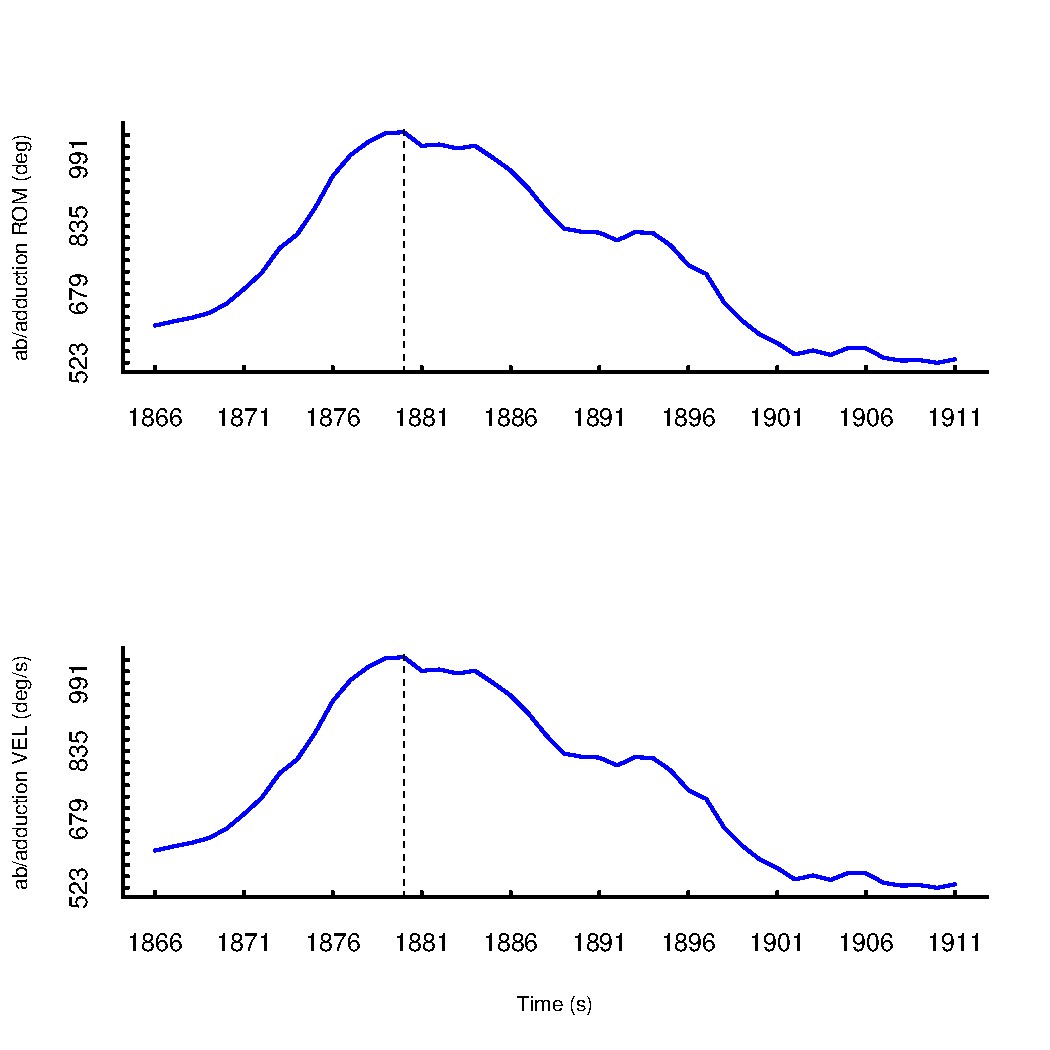
\includegraphics[width=4in,height=3in]{figure/latex-unnamed-chunk-1-1} \hfill{}



\end{knitrout}
\begin{knitrout}
\definecolor{shadecolor}{rgb}{0.969, 0.969, 0.969}\color{fgcolor}

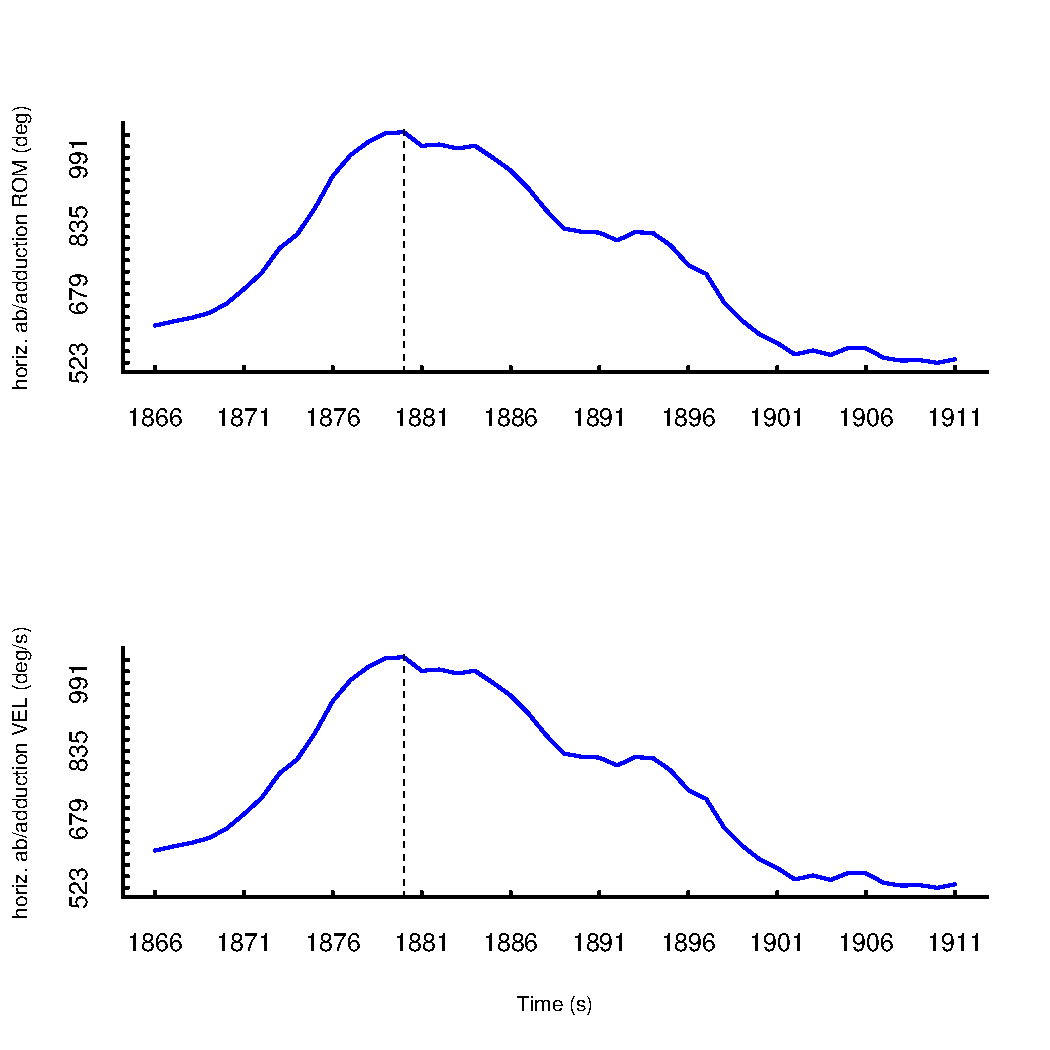
\includegraphics[width=4in,height=3in]{figure/latex-unnamed-chunk-2-1} \hfill{}



\end{knitrout}
\begin{knitrout}
\definecolor{shadecolor}{rgb}{0.969, 0.969, 0.969}\color{fgcolor}

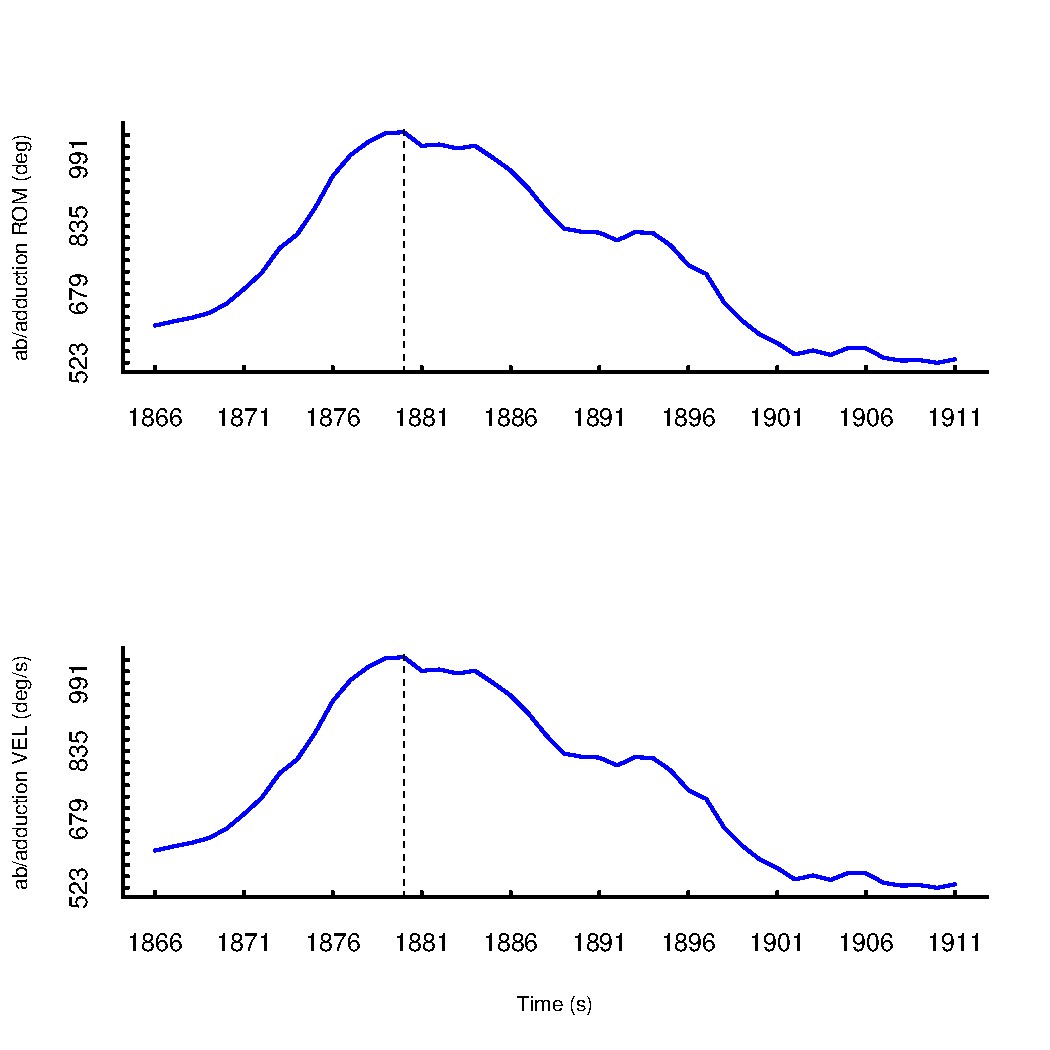
\includegraphics[width=4in,height=3in]{figure/latex-unnamed-chunk-3-1} \hfill{}



\end{knitrout}

\newpage

b. Neutral Posture Kinematics\\
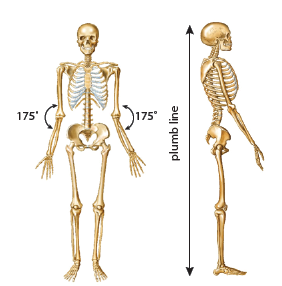
\includegraphics{SkeletonArmPosition.png}\\

\newpage

c. Pushup Dynamics
\begin{knitrout}
\definecolor{shadecolor}{rgb}{0.969, 0.969, 0.969}\color{fgcolor}

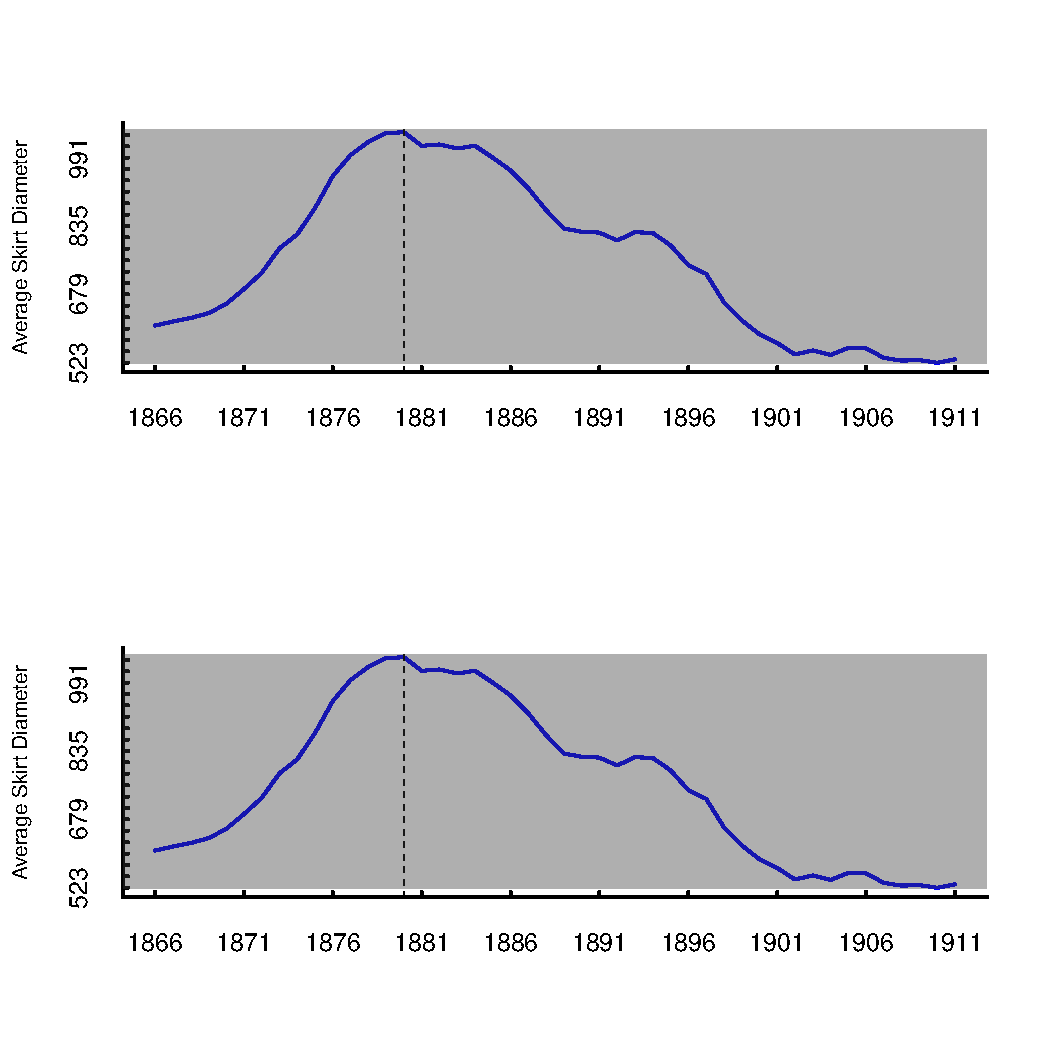
\includegraphics[width=4in,height=3in]{figure/latex-unnamed-chunk-4-1} \hfill{}



\end{knitrout}
d. Overhand Throw, one hand\\


e. Overhand Throw, two hand\\

\newpage

II. Lower Extremity\\
	a.Drop land

\begin{knitrout}
\definecolor{shadecolor}{rgb}{0.969, 0.969, 0.969}\color{fgcolor}

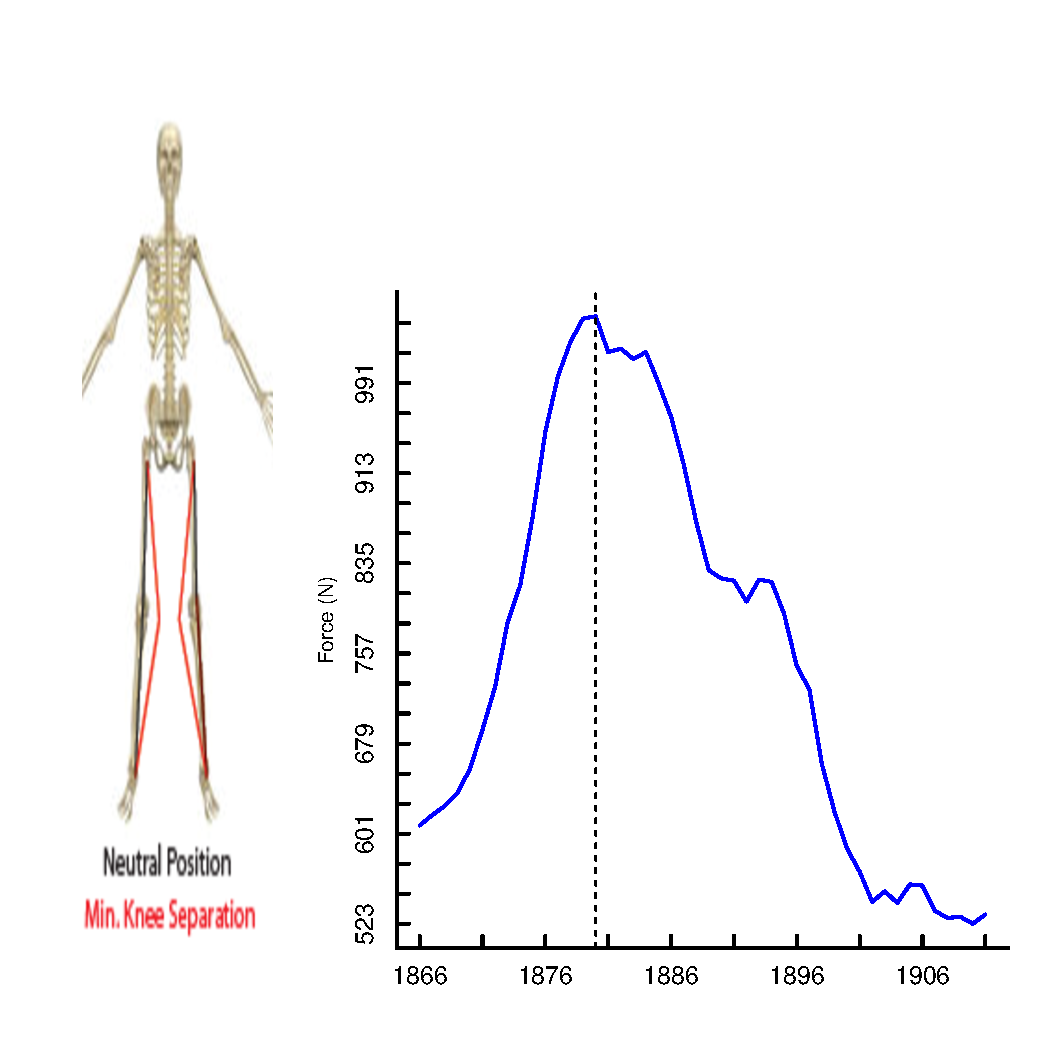
\includegraphics[width=6in,height=3in]{figure/latex-unnamed-chunk-5-1} \hfill{}



\end{knitrout}


\newpage


b. Drop Vertical Jump
\begin{knitrout}
\definecolor{shadecolor}{rgb}{0.969, 0.969, 0.969}\color{fgcolor}

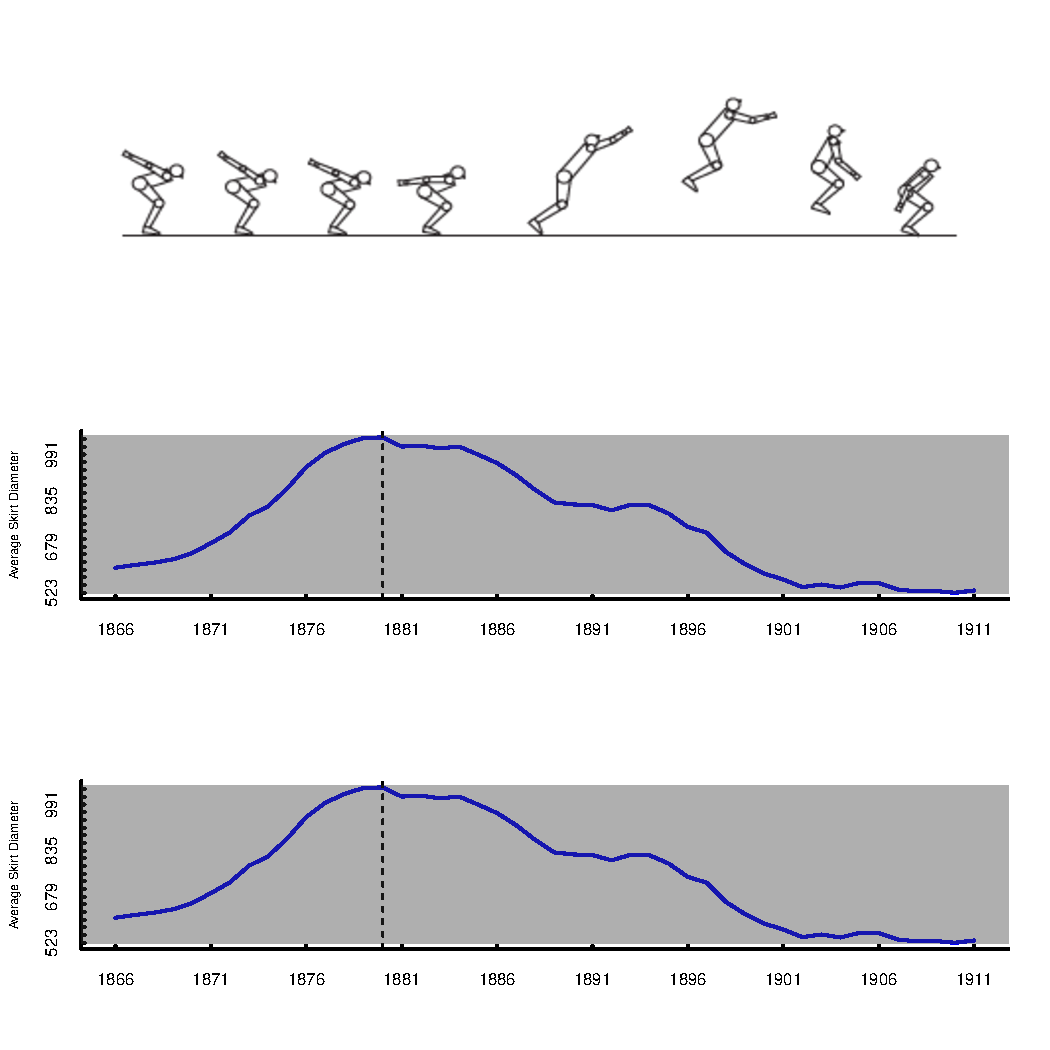
\includegraphics[width=5in,height=6in]{figure/latex-unnamed-chunk-6-1} \hfill{}



\end{knitrout}

\newpage

C. Standing Vertical Jump
\begin{knitrout}
\definecolor{shadecolor}{rgb}{0.969, 0.969, 0.969}\color{fgcolor}

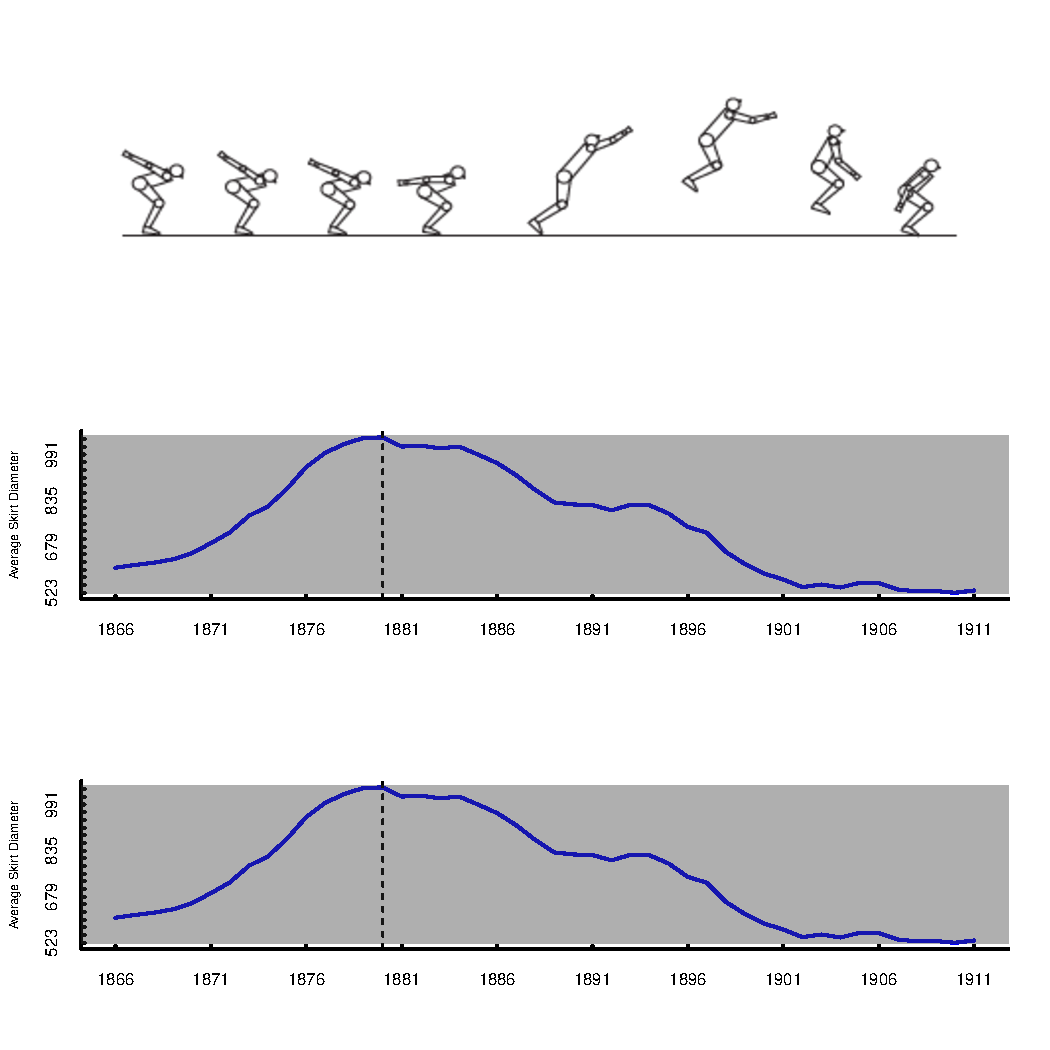
\includegraphics[width=5in,height=6in]{figure/latex-unnamed-chunk-7-1} \hfill{}



\end{knitrout}

\newpage
\
d.Approach Vertical Jump
\begin{knitrout}
\definecolor{shadecolor}{rgb}{0.969, 0.969, 0.969}\color{fgcolor}

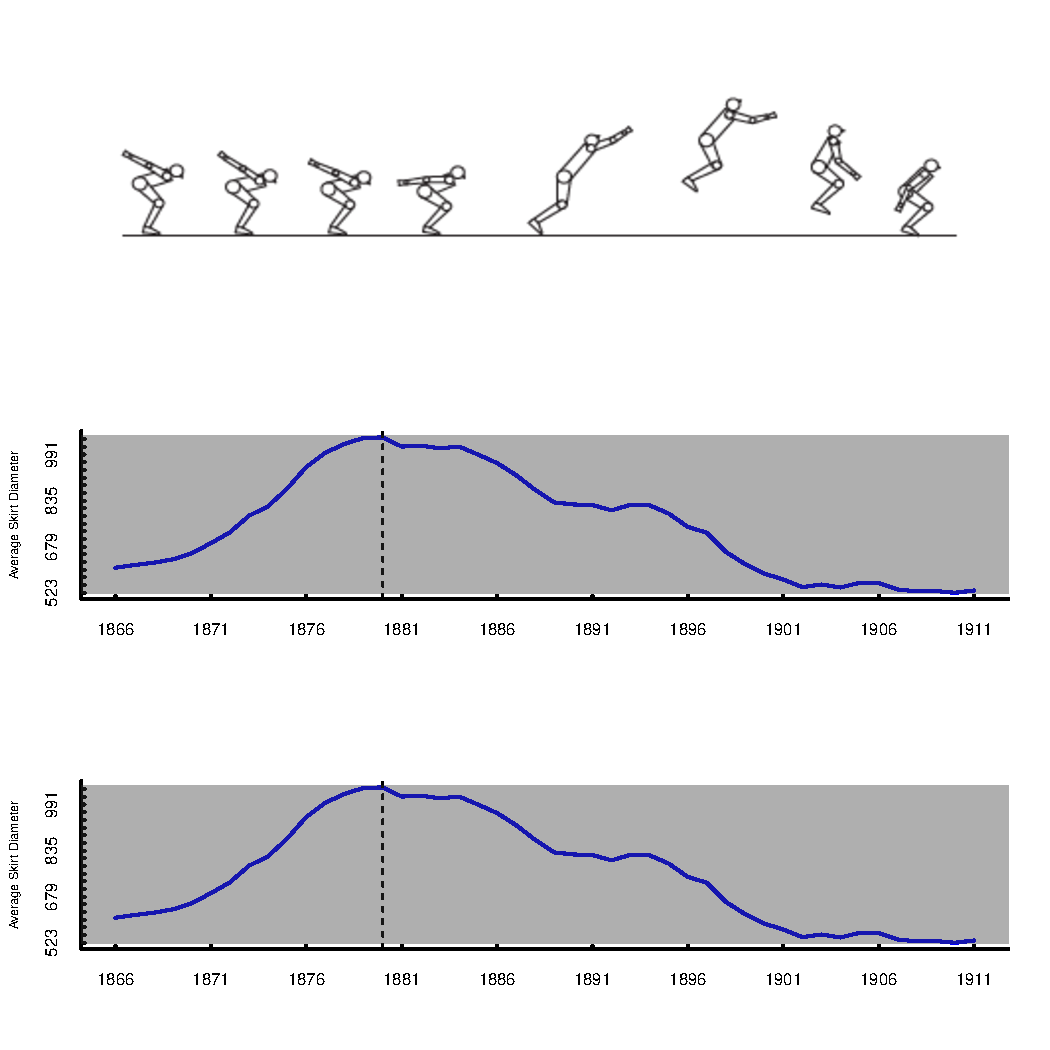
\includegraphics[width=5in,height=6in]{figure/latex-unnamed-chunk-8-1} \hfill{}



\end{knitrout}

e. Single Limb Balance
\begin{knitrout}
\definecolor{shadecolor}{rgb}{0.969, 0.969, 0.969}\color{fgcolor}

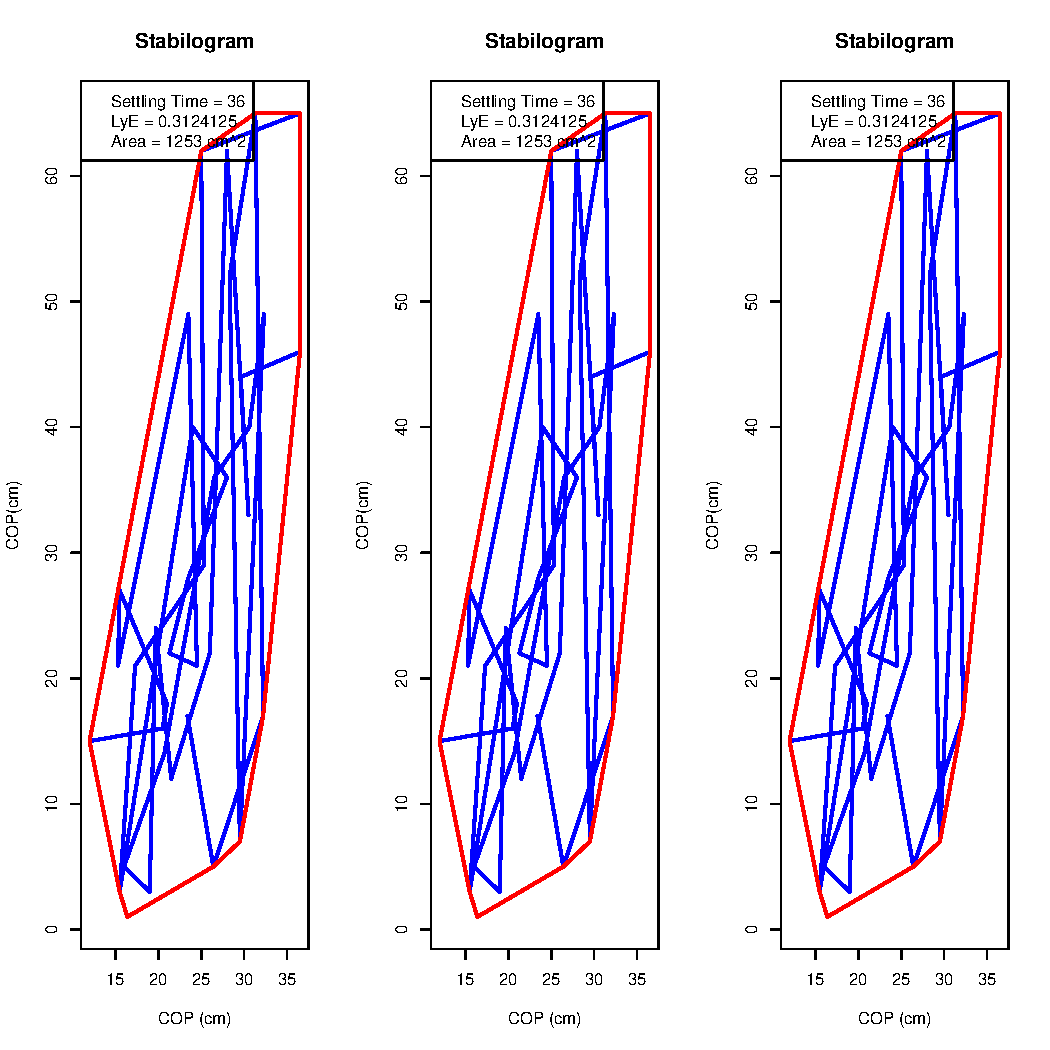
\includegraphics[width=6in,height=2in]{figure/latex-unnamed-chunk-9-1} \hfill{}



\end{knitrout}

\newpage

g. Cutting Mechanics\\
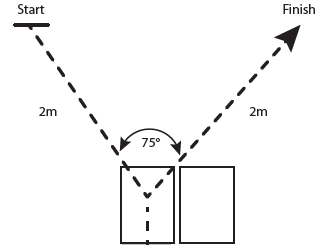
\includegraphics{StartFinishAngle.PNG}\\
\begin{knitrout}
\definecolor{shadecolor}{rgb}{0.969, 0.969, 0.969}\color{fgcolor}

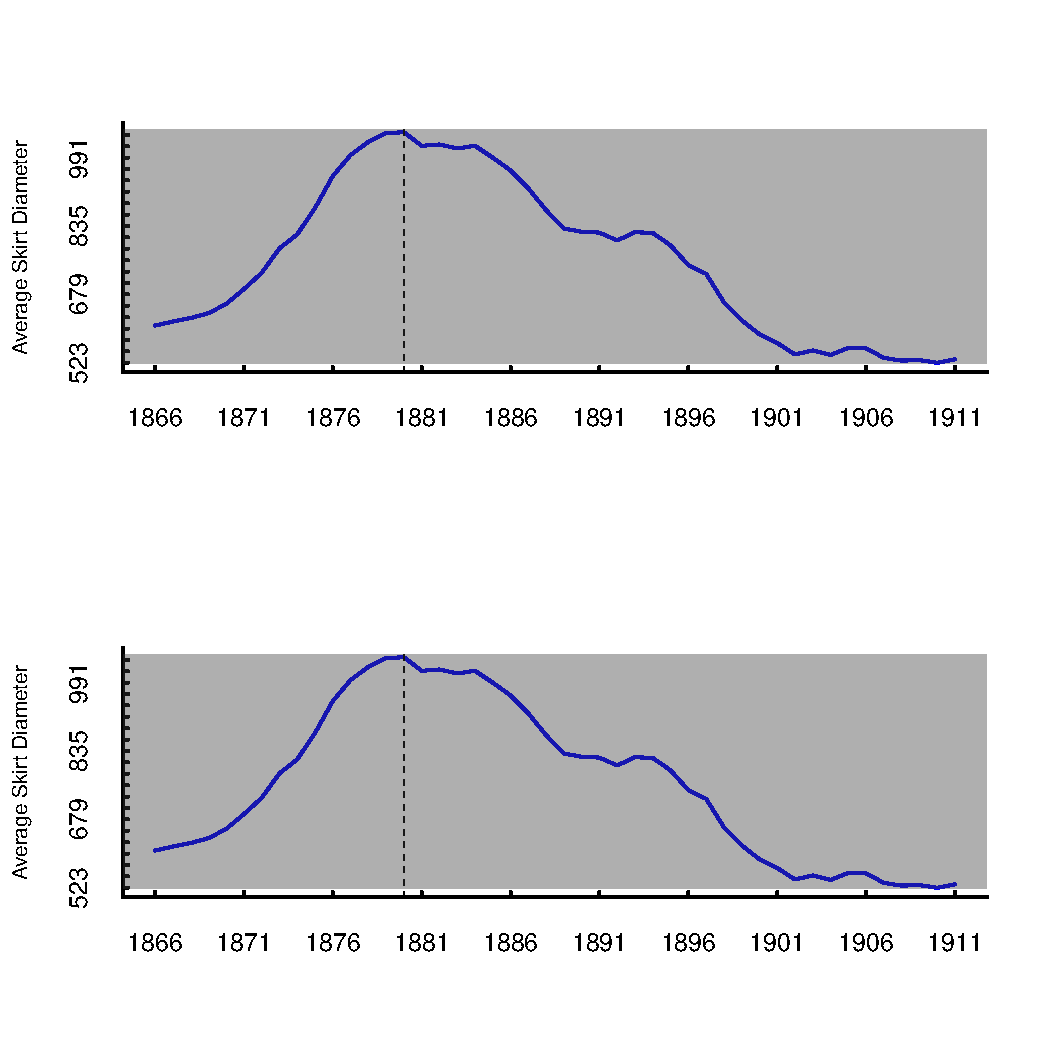
\includegraphics[width=5in,height=3in]{figure/latex-unnamed-chunk-10-1} \hfill{}



\end{knitrout}

\newpage
h. Single Limb Hop and Balance

\begin{knitrout}
\definecolor{shadecolor}{rgb}{0.969, 0.969, 0.969}\color{fgcolor}

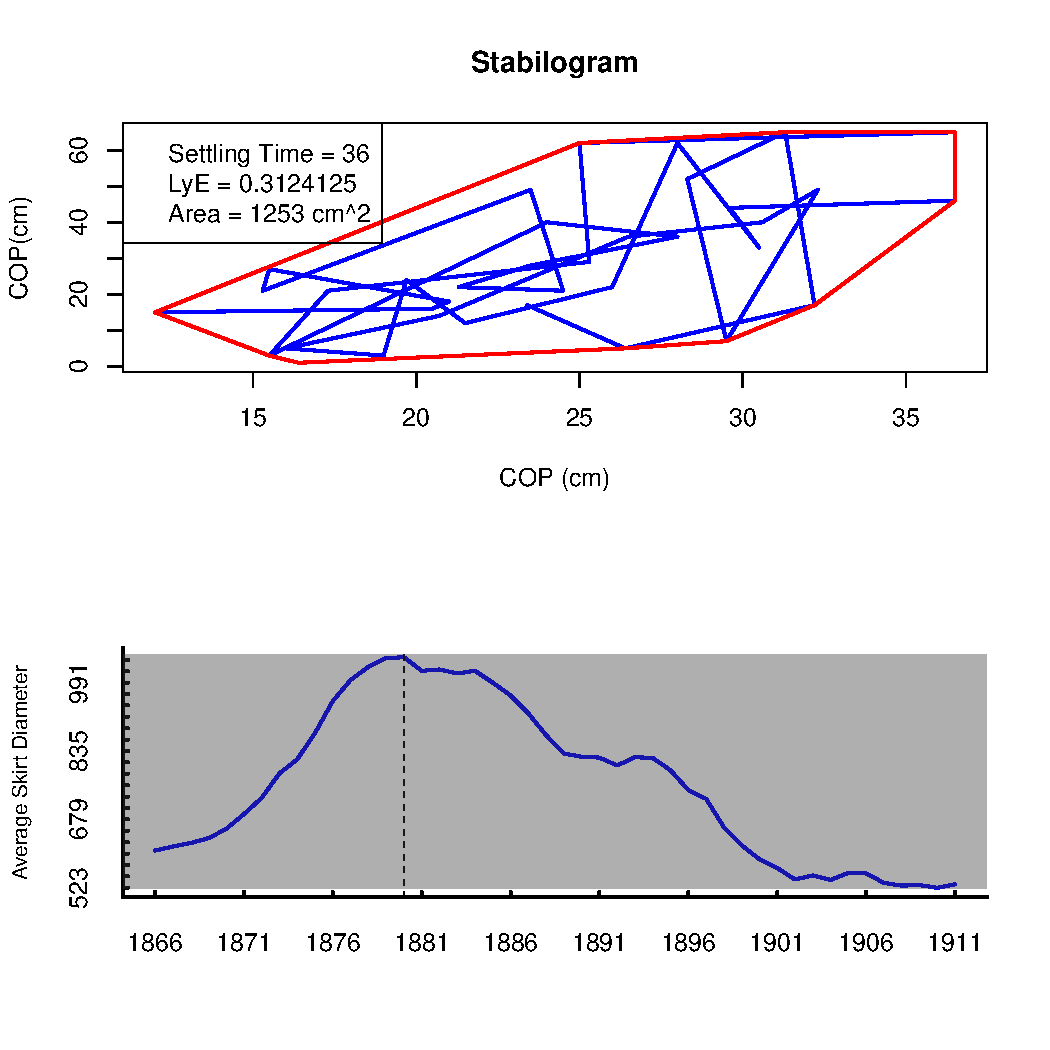
\includegraphics[width=6in,height=6in]{figure/latex-unnamed-chunk-11-1} \hfill{}



\end{knitrout}

i. Broad Jump
\begin{knitrout}
\definecolor{shadecolor}{rgb}{0.969, 0.969, 0.969}\color{fgcolor}

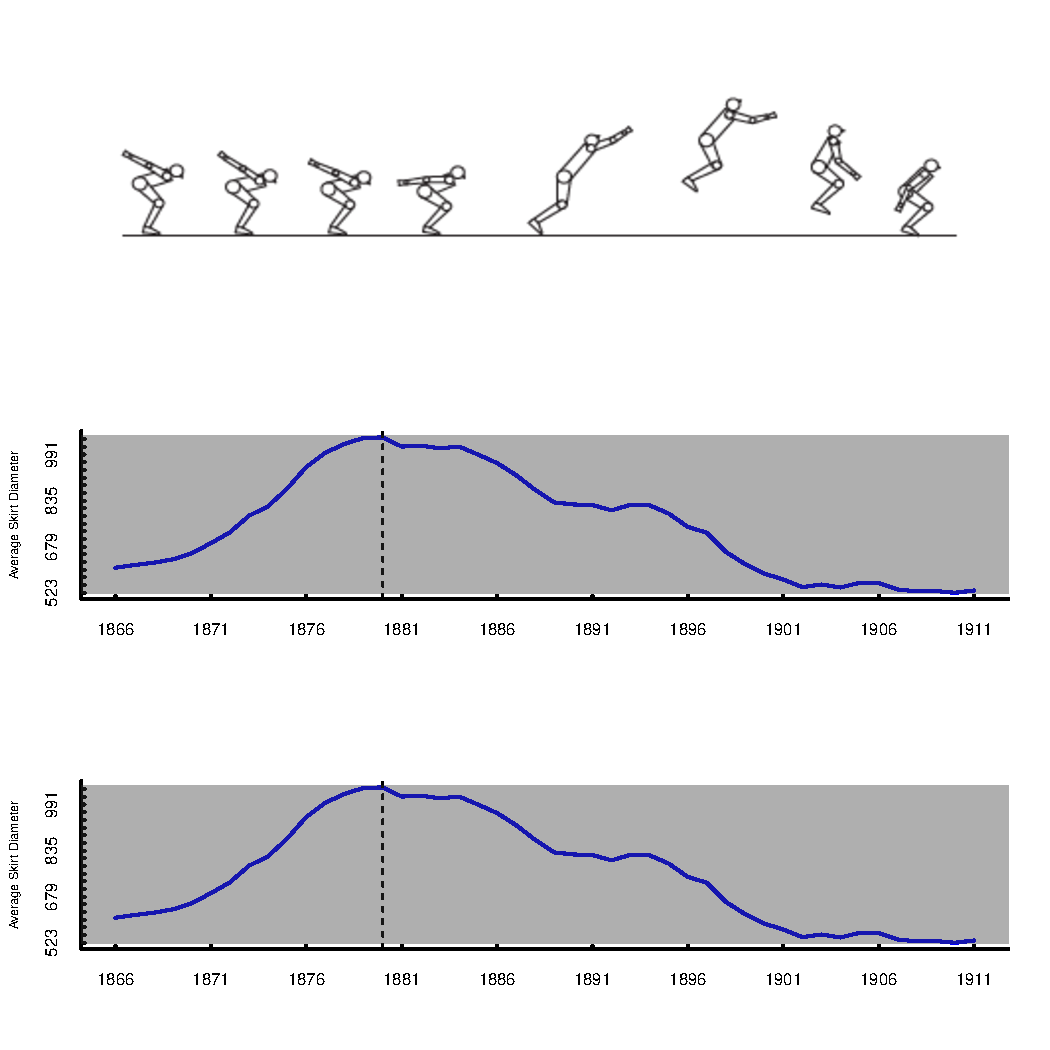
\includegraphics[width=6in,height=4in]{figure/latex-unnamed-chunk-12-1} \hfill{}



\end{knitrout}

J. Reaction Time

\begin{knitrout}
\definecolor{shadecolor}{rgb}{0.969, 0.969, 0.969}\color{fgcolor}

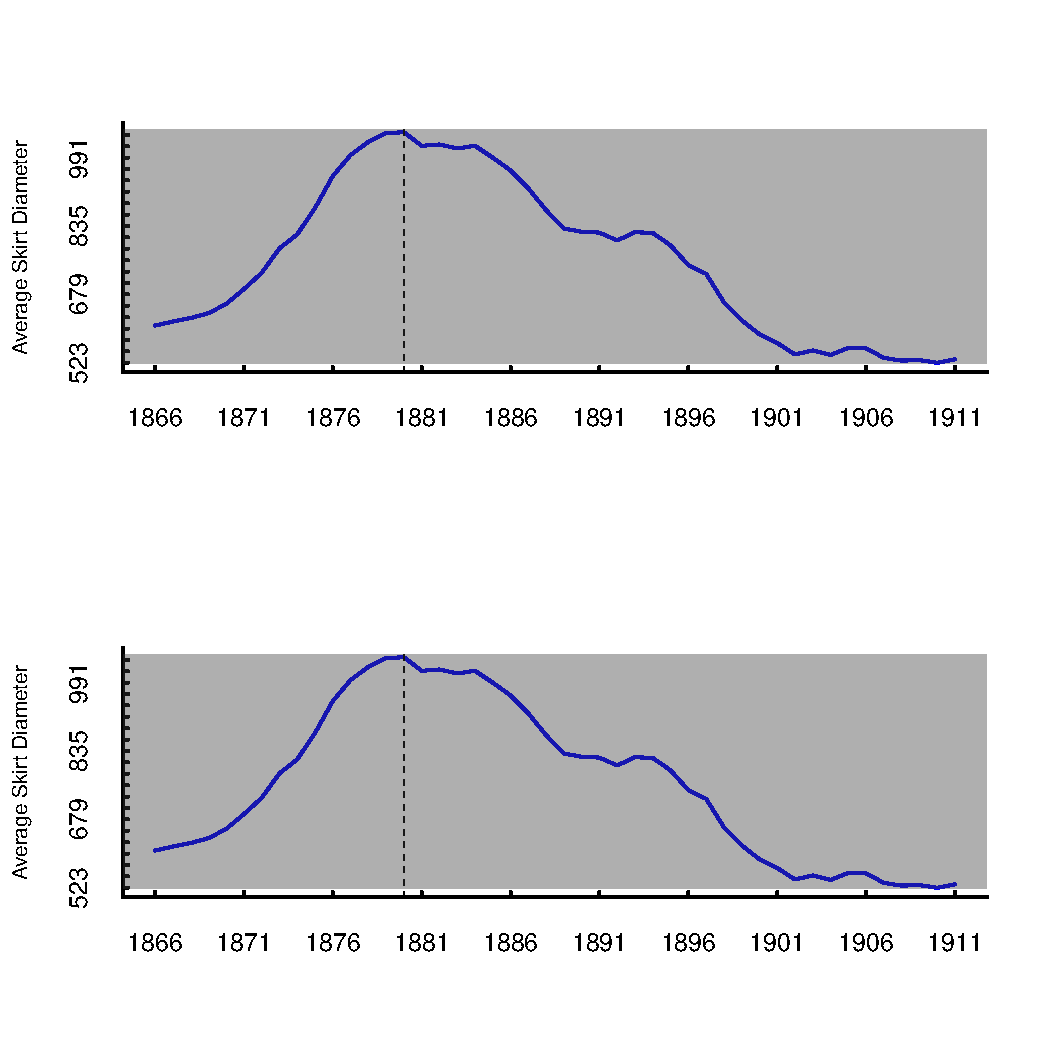
\includegraphics[width=6in,height=4in]{figure/latex-unnamed-chunk-13-1} \hfill{}



\end{knitrout}

\newpage

III. Core\\
a.Endurance 
\begin{knitrout}
\definecolor{shadecolor}{rgb}{0.969, 0.969, 0.969}\color{fgcolor}

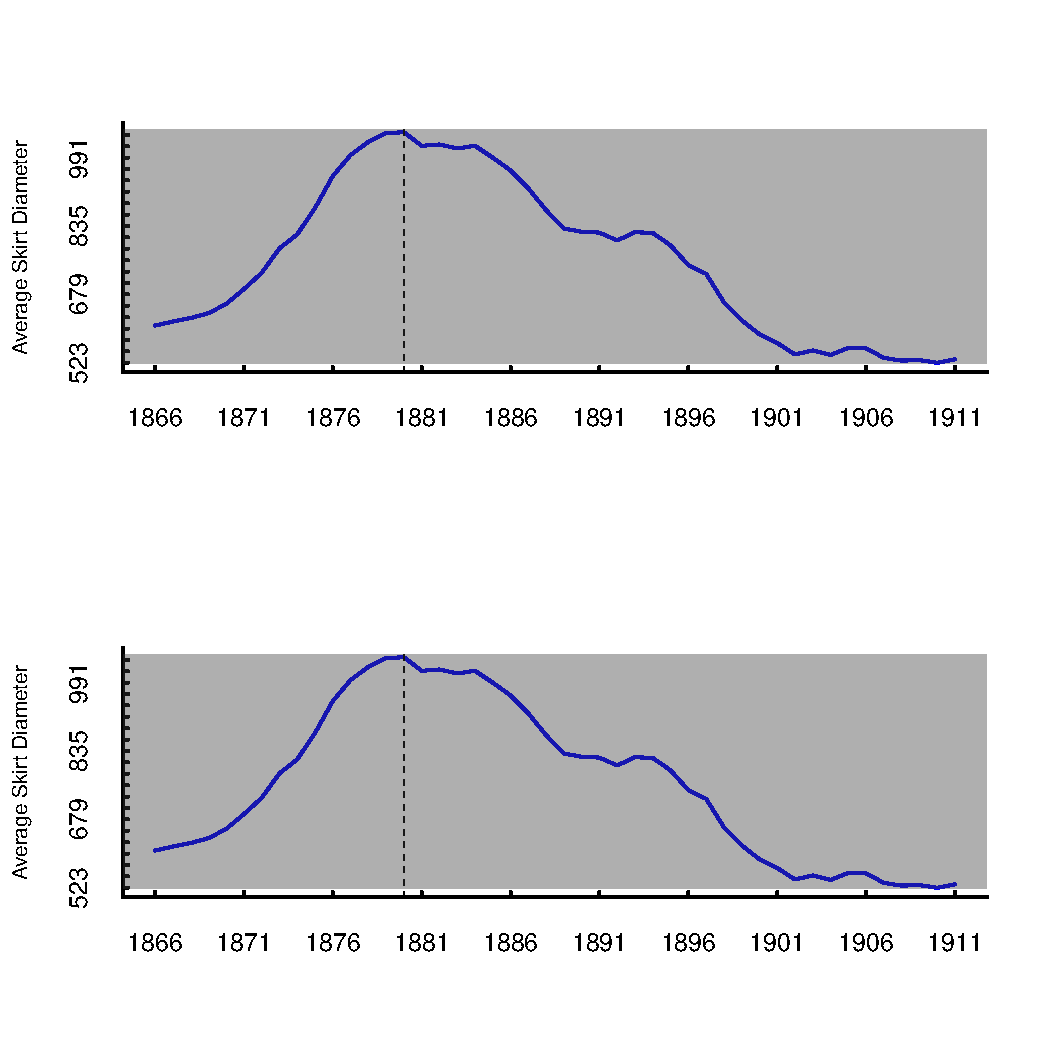
\includegraphics[width=6in,height=6in]{figure/latex-unnamed-chunk-14-1} \hfill{}



\end{knitrout}

\newpage
b.Explosive Power

\begin{knitrout}
\definecolor{shadecolor}{rgb}{0.969, 0.969, 0.969}\color{fgcolor}

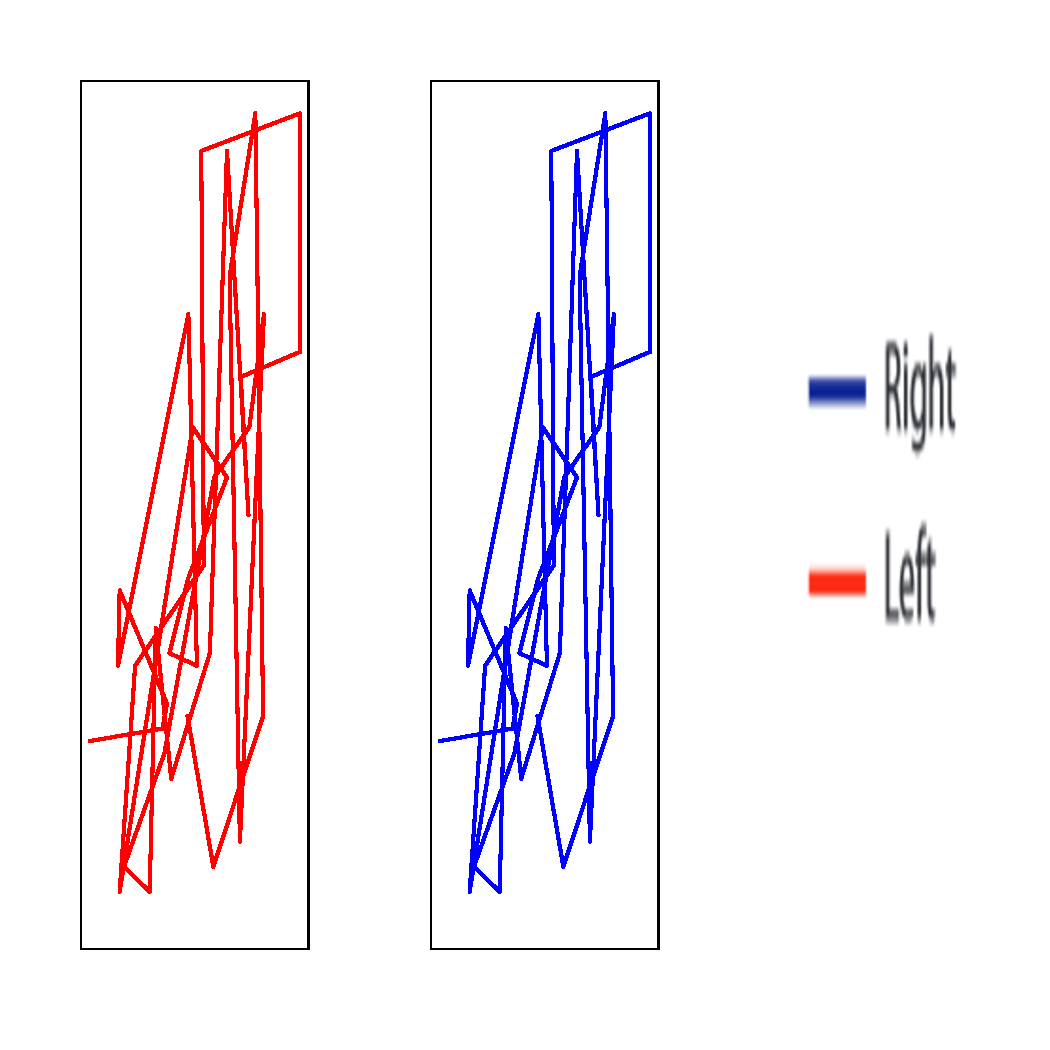
\includegraphics[width=6in,height=2in]{figure/latex-unnamed-chunk-15-1} \hfill{}



\end{knitrout}
\begin{knitrout}
\definecolor{shadecolor}{rgb}{0.969, 0.969, 0.969}\color{fgcolor}

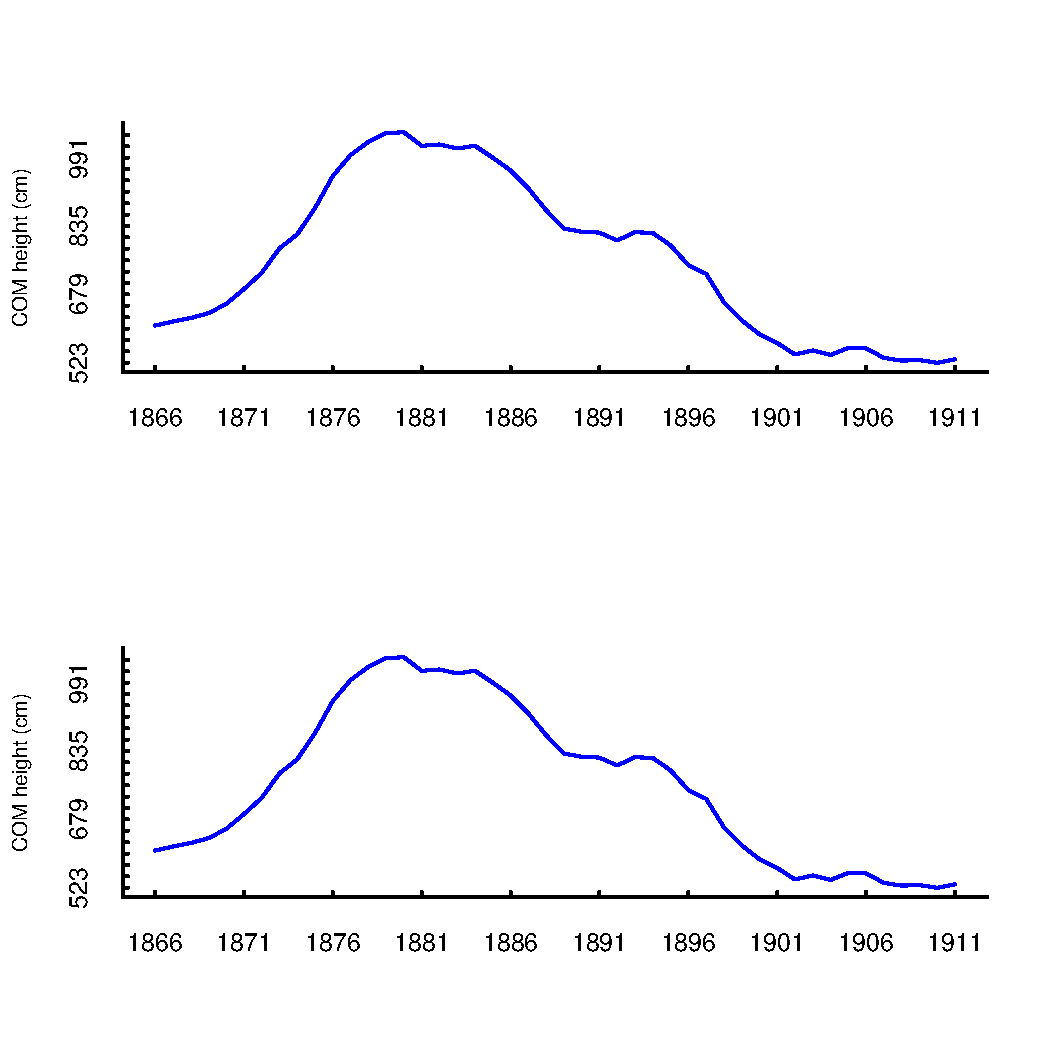
\includegraphics[width=6in,height=3in]{figure/latex-unnamed-chunk-16-1} \hfill{}



\end{knitrout}









\end{document}
